% Created 2015-11-28 Sat 11:54
\documentclass[a4paper]{tufte-handout}
\usepackage[scaled=0.95]{roboto}
\usepackage{mathpazo}
\linespread{1.05}
\usepackage{eulervm}
\usepackage[usenames]{xcolor}


%% footnote color 
\renewcommand{\thefootnote}{\textcolor{Gray}{\arabic{footnote}}}
\makeatletter

\renewcommand\@footnotetext[2][0pt]{%
  \marginpar{%
    \hbox{}\vspace*{#1}%
    \def\baselinestretch {\setspace@singlespace}%
    \reset@font\footnotesize%
    \@tufte@margin@par% use parindent and parskip settings for marginal text
    \vspace*{-1\baselineskip}\noindent%
    \protected@edef\@currentlabel{%
       \csname p@footnote\endcsname\@thefnmark%
    }%
    \color{Gray}
    \color@begingroup%
       \@makefntext{%
         \ignorespaces#2%
       }%
    \color@endgroup%
  }%
}%

\makeatother
%%==============================================================================
%%                                 SECTIONS
%%==============================================================================
%% section numbering to subsection
\setcounter{secnumdepth}{2}
\renewcommand{\thesection}{\Roman{section}}
\renewcommand{\thesubsection}{\thesection.\Alph{subsection}}
\renewcommand{\thesubsubsection}{\thesubsection\arabic{subsubsection})}
\renewcommand{\theparagraph}{\roman{paragraph}}
 
%%==============================================================================
%%                                 COLORS
%%==============================================================================
%% section format
\titleformat{\section}%
  {\normalfont\Huge\color{Cerulean}}% format applied to label+text
  {\llap{\colorbox{Cerulean}{\parbox{1.5cm}{\hfill\color{white}\thesection}}}}% label
  {1em}% horizontal separation between label and title body
  {}% before the title body
  []% after the title body

% subsection format
\titleformat{\subsection}%
  {\normalfont\Large\itshape\color{TealBlue}}% format applied to label+text
  {\llap{\colorbox{TealBlue}{\parbox{1cm}{\hfill\color{white}\thesubsection}}}}% label
  {0.5em}% horizontal separation between label and title body
  {}% before the title body
  []% after the title body

\renewcommand{\footnotesize}{\scriptsize}
\setcaptionfont{\color{Gray}\footnotesize}
\setsidenotefont{\color{Gray}\footnotesize}
\setmarginnotefont{\color{Gray}\itshape\footnotesize}

\usepackage[utf8]{inputenc}
\usepackage[T1]{fontenc}
\usepackage{graphicx}
\usepackage{longtable}
\usepackage{float}
\usepackage{hyperref}
\usepackage{wrapfig}
\usepackage{rotating}
\usepackage[normalem]{ulem}
\usepackage{amsmath}
\usepackage{textcomp}
\usepackage{marvosym}
\usepackage{wasysym}
\usepackage{amssymb}
\usepackage[scaled=0.9]{zi4}
\usepackage[usenames, dvipsnames]{xcolor}
\usepackage[protrusion=true, expansion=alltext, tracking=true, kerning=true]{microtype}
\usepackage{siunitx}
\usepackage[frenchle, frenchb]{babel}
\usepackage{biolinum}
\usepackage[euler-digits]{eulervm}
\renewcommand{\footnotesize}{\small}
\author{Samuel BARRETO}
\date{\today}
\title{Premières Analyses des Données de Séquençage}
\hypersetup{
 pdfauthor={Samuel BARRETO},
 pdftitle={Premières Analyses des Données de Séquençage},
 pdfkeywords={},
 pdfsubject={},
 pdfcreator={Emacs 24.5.1 (Org mode 8.3.2)}, 
 pdflang={Frenchb}}
\begin{document}

\maketitle

\section{Qualité des données}
\label{sec:orgheadline4}
\subsection{qualité du séquençage}
\label{sec:orgheadline1}
\begin{marginfigure}
  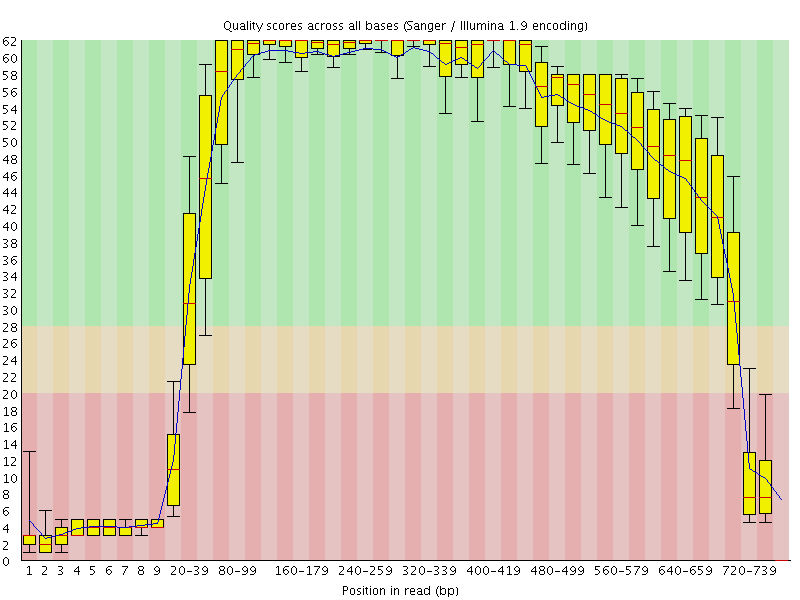
\includegraphics[width=\linewidth]{../per_base_quality_fastqc_untrimmed.png}
  \caption{Qualité des séquences \emph{avant} d'être trimmées et filtrées
      sur la qualité}
\end{marginfigure}

\begin{marginfigure}
  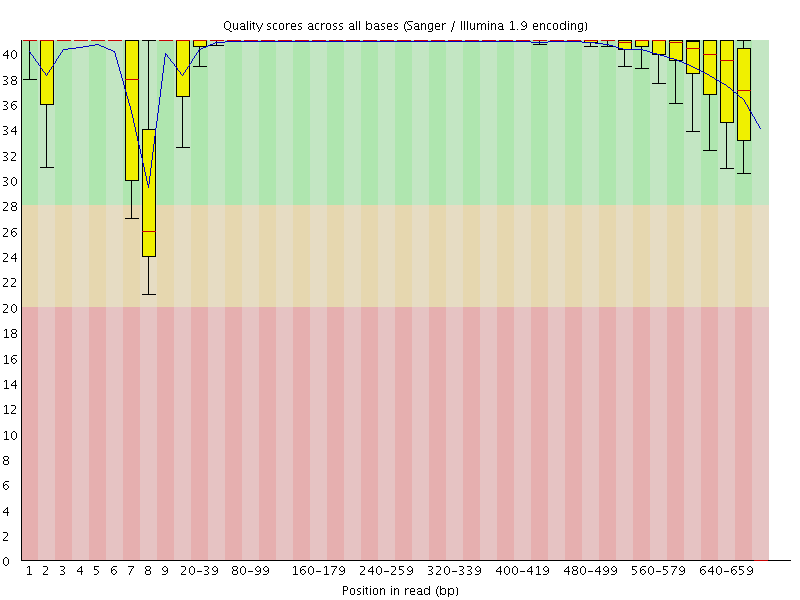
\includegraphics[width=\linewidth]{../per_base_quality_fastqc_trimmed.png}
  \caption{Qualité des séquences \emph{après} avoir été trimmées et filtrées
      sur la qualité}
\end{marginfigure}

Globalement la plupart des séquences était de bonne qualité. Sur les \(192\)
envoyées à séquencer, \(170\) ont été retenues pour l'analyse, soit \(89\) \%.

Étant donnée la faible qualité des bases en début et en fin de séquence, elles
ont été tronquées. Le score \(28\) semblait le seuil naturel de qualité. De plus,
toutes les séquences qui avaient une longueur inférieure à \(620\) étaient
généralement mal alignées. Elles ont été éliminées de l'analyse. 

Il reste au final \(83\) séquence de Strong et \(87\) séquences de Weak. 

\subsection{Présence de contaminations ?}
\label{sec:orgheadline2}

\begin{center}
\small
\begin{tabular}{ccc}
\toprule
 & \textbf{SNP weak} & \textbf{SNP strong}\\
\midrule
pS60-1073 & 22 & \\
pS83-1073 & 21 & \\
pS91-1073 & 22 & \\
pS92-1073 & 22 & \\
pW6-1073 &  & 10\\
\bottomrule
\end{tabular}
\end{center}

Toutes ces séquences ont été ``rebasculées'' dans la catégorie qui leur
convient. 
\subsection{Observations générales}
\label{sec:orgheadline3}

\begin{margintable}
  \small
  
\begin{tabular}{cccc}
\toprule
mutant & mean & med & sd\\
\midrule
strong & 14.89 & 15 & 6.13\\
weak & 13.70 & 13 & 6.28\\
\bottomrule
\end{tabular}

\end{margintable}

Il y a \(1236\) SNP générés par l'exogène Strong, et \(1192\) SNP générés par l'exogène
Weak. \\
\begin{center}
  
\begin{tabular}{cc}
\toprule
Type de mutation & nombre\\
\midrule
SW & 1188\\
WS & 1237\\
WW & 3\\
\bottomrule
\end{tabular}

\end{center}

\newpage
\section{Distribution des SNPs}
\label{sec:orgheadline7}
\subsection{Distribution globale}
\label{sec:orgheadline5}
\begin{figure*}[h]
  \centering
  \includegraphics[width=\linewidth]{../snp_distribution.pdf}
  \caption{La distibution des SNPs, sans tenir compte de la qualité de la
    mutation. La couleur représente le mutant d'origine.}
  \label{fig:snpdistrib}
\end{figure*}

Ce graphe représente la distribution des SNPs sur la séquence de référence. Les
barres vertes représentent les SNP des gènes synthétiques Strong, les rouges
celles des Weak. 

Première observation : il y a plus de SNP dans les régions 5' que 3'. Artefact
de séquençage ? Quand on regarde la qualité du \emph{base call} et les spectrogrammes
associés, il ne semble pas. 

Deuxième observation : les gènes synthétiques Strong génèrent \emph{légèrement} plus
de SNPs en 3' que les Weak. À tester, pas certain que ce soit significatif.

\newthought{Conclusion} : il y a plus de substitutions dans les régions 3' que 5',
sur la fin de la conversion tract. Où se fait le switch ? 

\marginnote{ À noter qu'on n'a pas de SNP après la position 691, alors que la
  séquence de référence mesure $734$bp. C'est dû au \emph{trimming} des
  séquences. On perd l'information des premiers SNP. }

\newpage
\subsection{Distribution de la qualité des mutation}
\label{sec:orgheadline6}

\begin{figure*}[h]
  \centering
  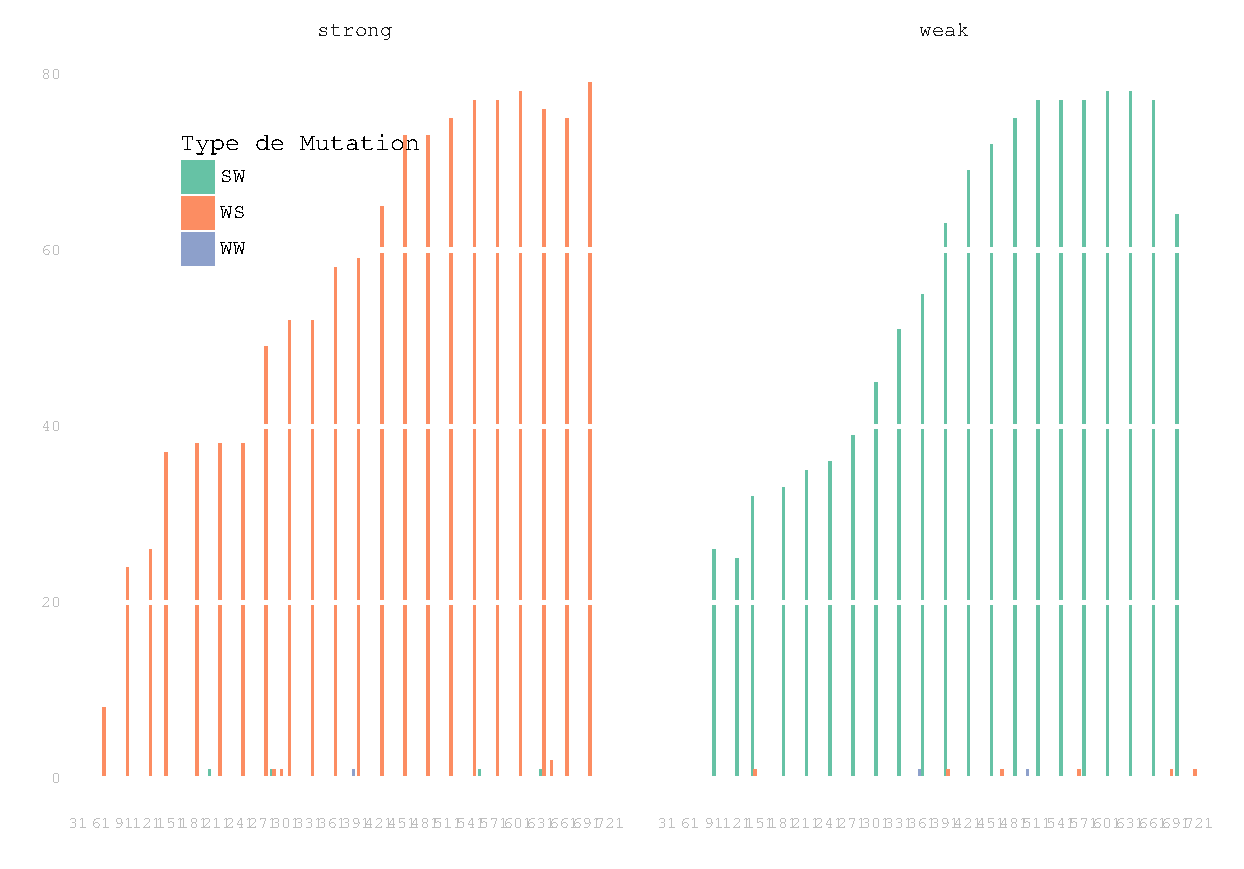
\includegraphics[width=\linewidth]{../mutant_snp_distribution.pdf}
  \caption{\textbf{Distribution des SNP par position sur la séquence de référence.} \\
    On retrouve bien les positions des polymorphismes ``artificiels'', toutes
    les $30$ paires de bases. En vert les mutations \emph{strong} et en rouge
    les mutations \emph{weak}. Les mutants Strong montrent quasiment
    exclusivement des substitutions \emph{strong}. Les mutants Weak montrent
    aussi exclusivement des substitutions \emph{weak}. }
  \label{fig:mutsnpdistrib}
\end{figure*}

En haut, la distribution des SNP générés par les gènes synthétiques de type
Strong ; en bas, celle des gènes synthétiques de type Weak. Les barres rouges 
représentent les substitutions vers \(GC\), \emph{strong} ; les barres vertes les
substitutions vers \(AT\), \emph{weak}, les quelques barres bleues --- il y en a trois
--- représentent les mutations spontanées \(WW\). 

Lorsque le gène synthétique est de type Strong, les substitutions occasionnées
sont --- quasiment --- exclusivement de type \emph{strong} ; idem pour les gènes
synthétiques Weak. 

\clearpage
\section{Distribution de la position de basculement}
\label{sec:orgheadline9}
\subsection{Basculement terminal global}
\label{sec:orgheadline8}
\begin{figure*}
  \centering
  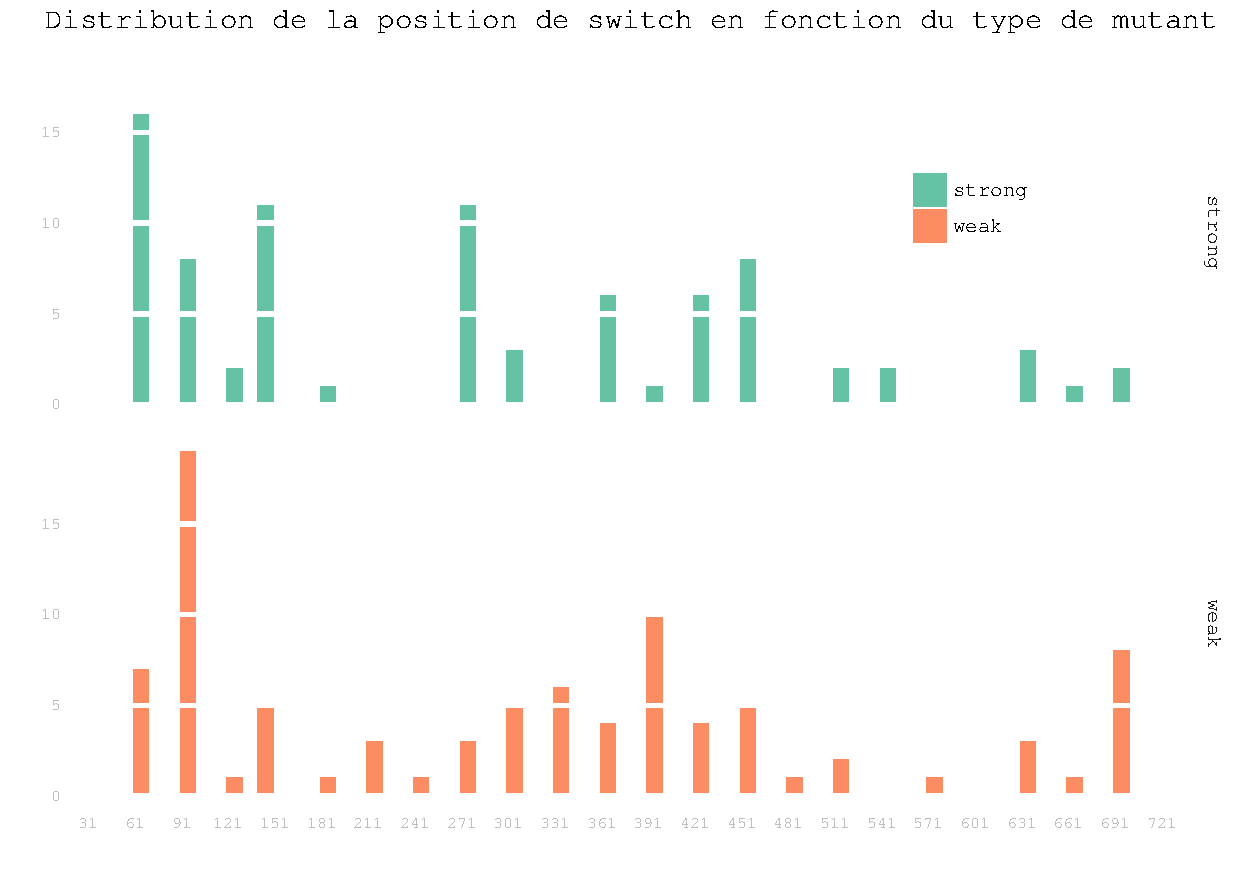
\includegraphics[width=\linewidth]{../switch_distrib.pdf}
  \caption{\textbf{Position des switch, indifféremment de la qualité de la
      substition ou du mutant}. \\
    Il y a des disparités dans la distribution des positions de basculement. Il
    y a beaucoup de basculement dès le début, moins vers la fin. Il semble y
    avoir une sorte de \emph{coldspot} local, autour de $500$bp et $200$bp sur
    la séquence de référence. }
\end{figure*}

Ce graphe représente la distribution du dernier SNP par mutant : autrement dit,
la position de basculement. Il y a une très forte hétérogénéité. Peut-on parler
de coldspot / hotspot local ?

On ne voit pas de divergence très nette entre l'haplotype Weak et l'haplotype
Strong, mis à part peut-être le pic dans les premiers SNP, plus fort pour le
Weak\ldots

\newpage
\section{Le BGC en action ?}
\label{sec:orgheadline10}

\begin{figure}
  \centering
  \includegraphics[width=\linewidth]{../bgc_en_action.pdf}
  \caption{\textbf{Distribution des SNPs aux positions non-calibrées}}
  \label{fig:bgcenaction}
\end{figure}

Voilà ce que je vois : si on n'observe que les positions qui ne sont pas celles
attendues, les substitutions sont en faveur de GC. Au contraire, lorsqu'on
regarde les positions ``calibrées'', on a \textbf{toujours} le SNP attendu. 
\begin{center}
  {\sffamily % latex table generated in R 3.2.2 by xtable 1.8-0 package
% Thu Dec  3 18:39:36 2015
\begin{table}[ht]
\centering
\begin{tabular}{cc}
  \hline
Type de Substitution & Nombre \\ 
  \hline
SW &   3 \\ 
  WS &  12 \\ 
  WW &   3 \\ 
   \hline
\end{tabular}
\end{table}
}
\end{center}

\begin{figure}
  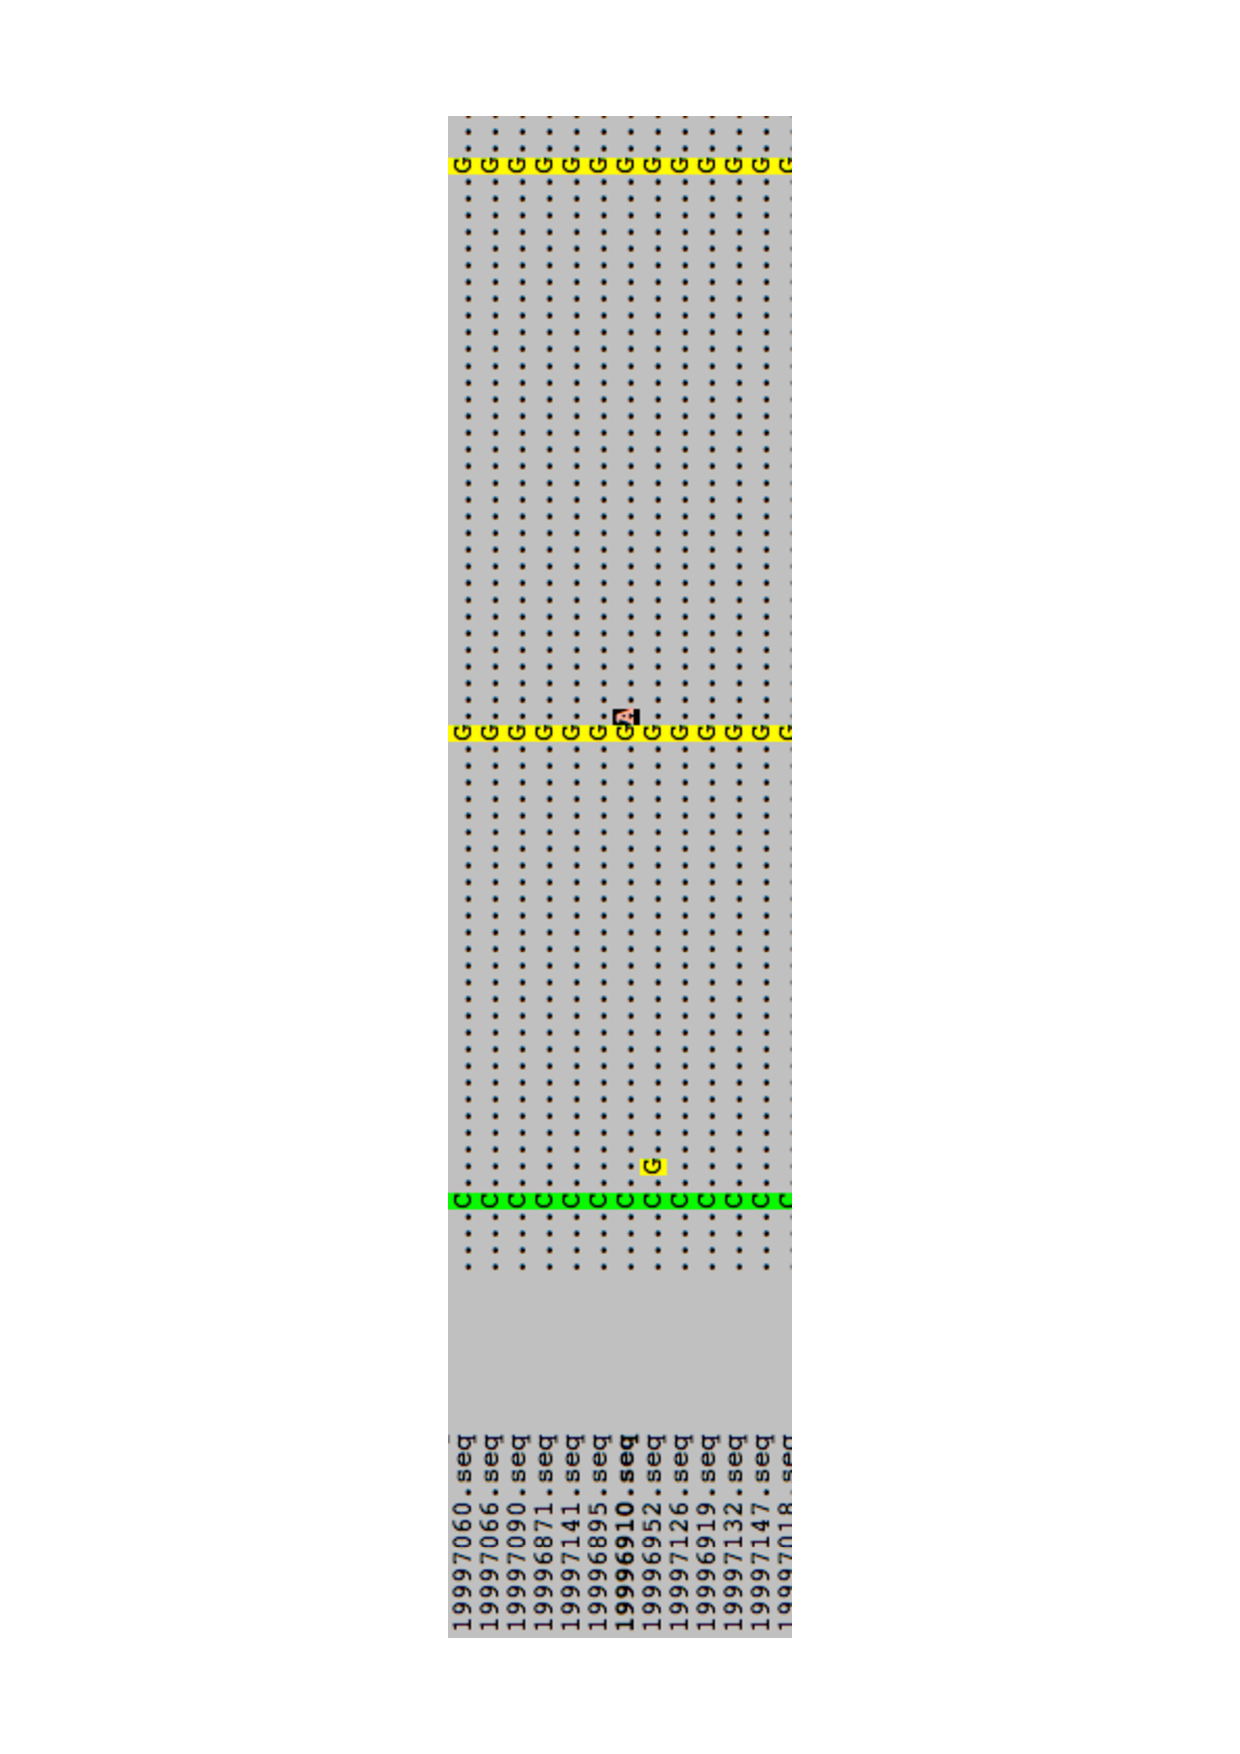
\includegraphics[width=\linewidth]{../inattendu.png}
  \caption{Bon, sauf dans le cas de {\em ce} mutant, je n'ai pas jugé nécessaire
    de réécrire toutes mes fonctions pour un SNP. Son cas est quand même bien
    curieux…}
\end{figure}
\end{document}